\documentclass[11pt,a4paper]{article}

\usepackage[margin=2.2cm]{geometry}
\usepackage[T1]{fontenc}
\usepackage[utf8]{inputenc}
\usepackage{lmodern}
\usepackage{microtype}
\usepackage{graphicx}
\usepackage{float}
\usepackage{booktabs}
\usepackage{tabularx}
\usepackage{array}
\usepackage{longtable}
\usepackage{hyperref}
\usepackage{xcolor}
\usepackage{enumitem}

\hypersetup{
  colorlinks=true,
  linkcolor=blue!45!black,
  urlcolor=blue!45!black
}

\setlength{\parindent}{0pt}
\setlength{\parskip}{0.35em}
\setlength{\textfloatsep}{0.5em}
\setlength{\floatsep}{0.5em}
\setlength{\intextsep}{0.5em}
\setlength{\abovecaptionskip}{4pt}
\setlength{\belowcaptionskip}{0pt}
\renewcommand{\arraystretch}{1.22}
\graphicspath{{figures/}{../results/}}
\setlist{itemsep=0.2em, topsep=0.3em, parsep=0pt, partopsep=0pt}

\newcolumntype{Y}{>{\raggedright\arraybackslash}X}
\newcommand{\code}[1]{\texttt{#1}}

\title{\textbf{Coin Classification with AlexNet}\\[0.4em]}

\author{Mehdi AGHAEI - VMI}
\date{March 22, 2026}

\begin{document}
\maketitle


\section{Dataset Audit}
The training annotations contain 10,368 rows. After removing corrupted files, 10,365 training images remain usable. The test split contains 1,282 images, and the cleaned training set covers 315 classes. The corrupted training files detected during the audit are \code{10211}, \code{11270}, and \code{11353}. Detecting them before training is important because unreadable files can interrupt a run or silently corrupt preprocessing.

The dataset is clearly imbalanced. Some classes contain only 13 examples, whereas the largest classes contain up to 108 images. This class imbalance means that top-1 accuracy alone is not sufficient to judge the model fairly. For that reason, the pipeline reports top-5 accuracy, macro-F1, and balanced accuracy in addition to the usual validation accuracy.

This dataset structure strongly motivates several later design decisions: stratified validation splitting, weighted sampling during training, transfer learning instead of training from scratch, and regularization mechanisms such as label smoothing.

\begin{figure}[htbp]
    \centering
    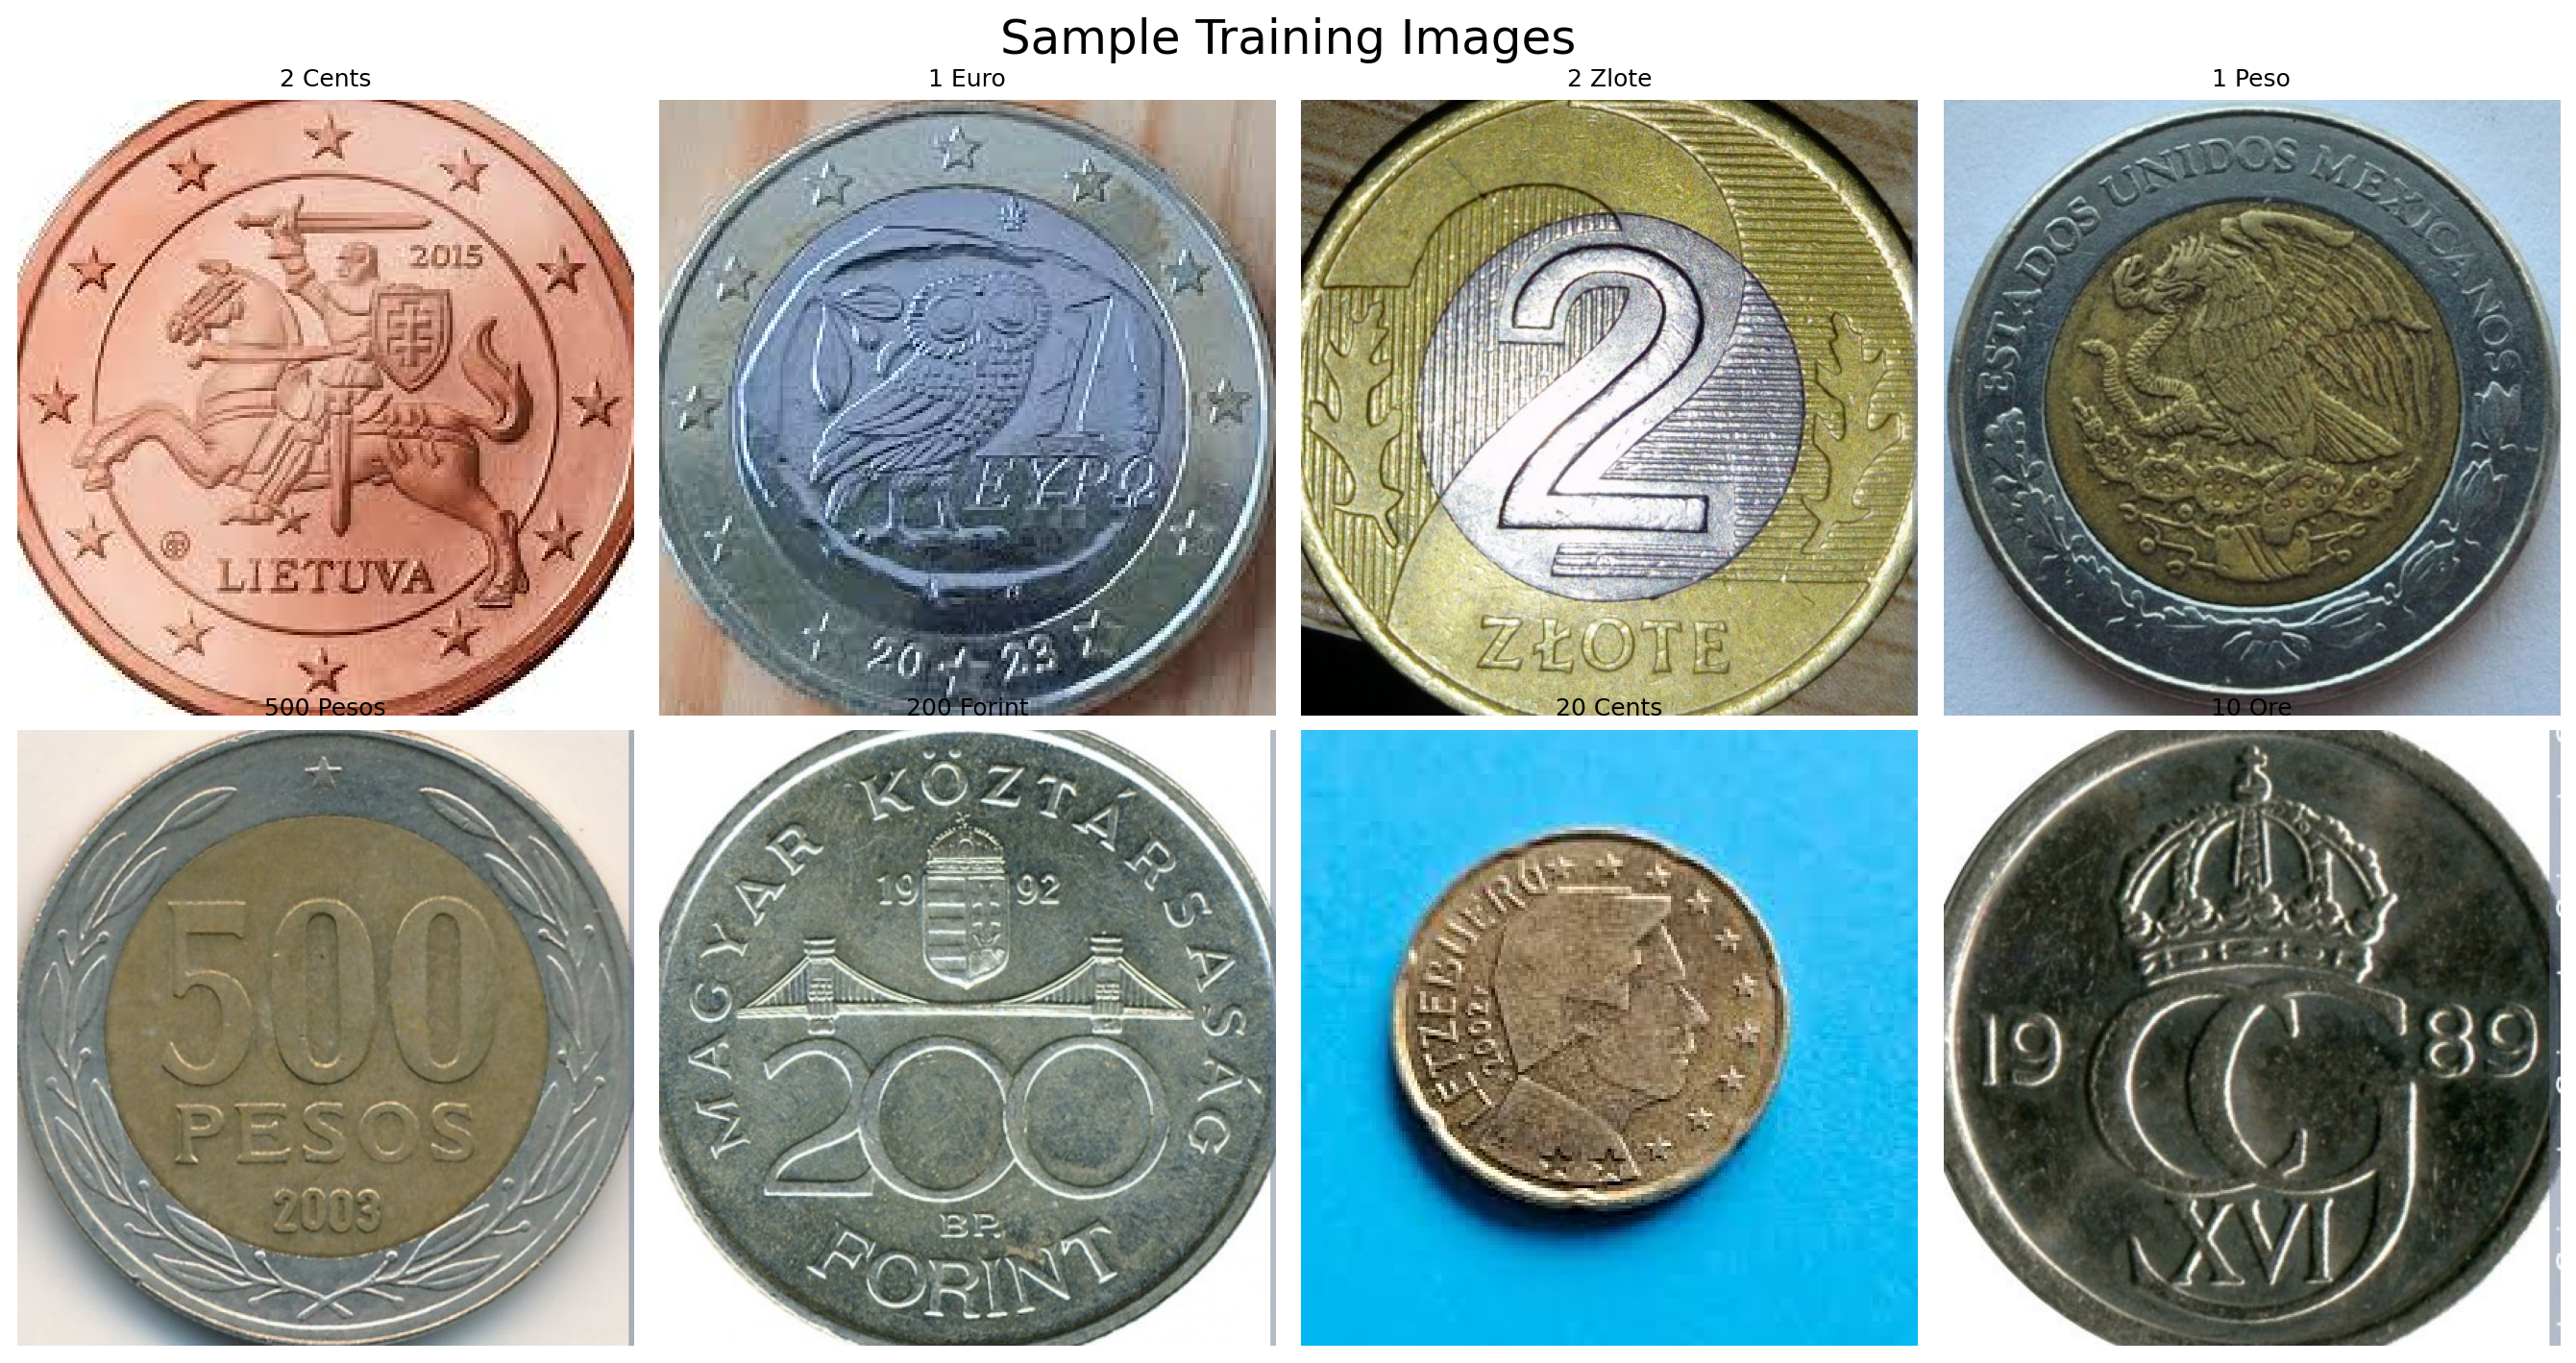
\includegraphics[width=\textwidth]{sample_gallery.png}
    \caption{Representative training images from the coin dataset. The fine-grained visual differences between classes make transfer learning and careful augmentation necessary.}
\end{figure}

\begin{figure}[htbp]
    \centering
    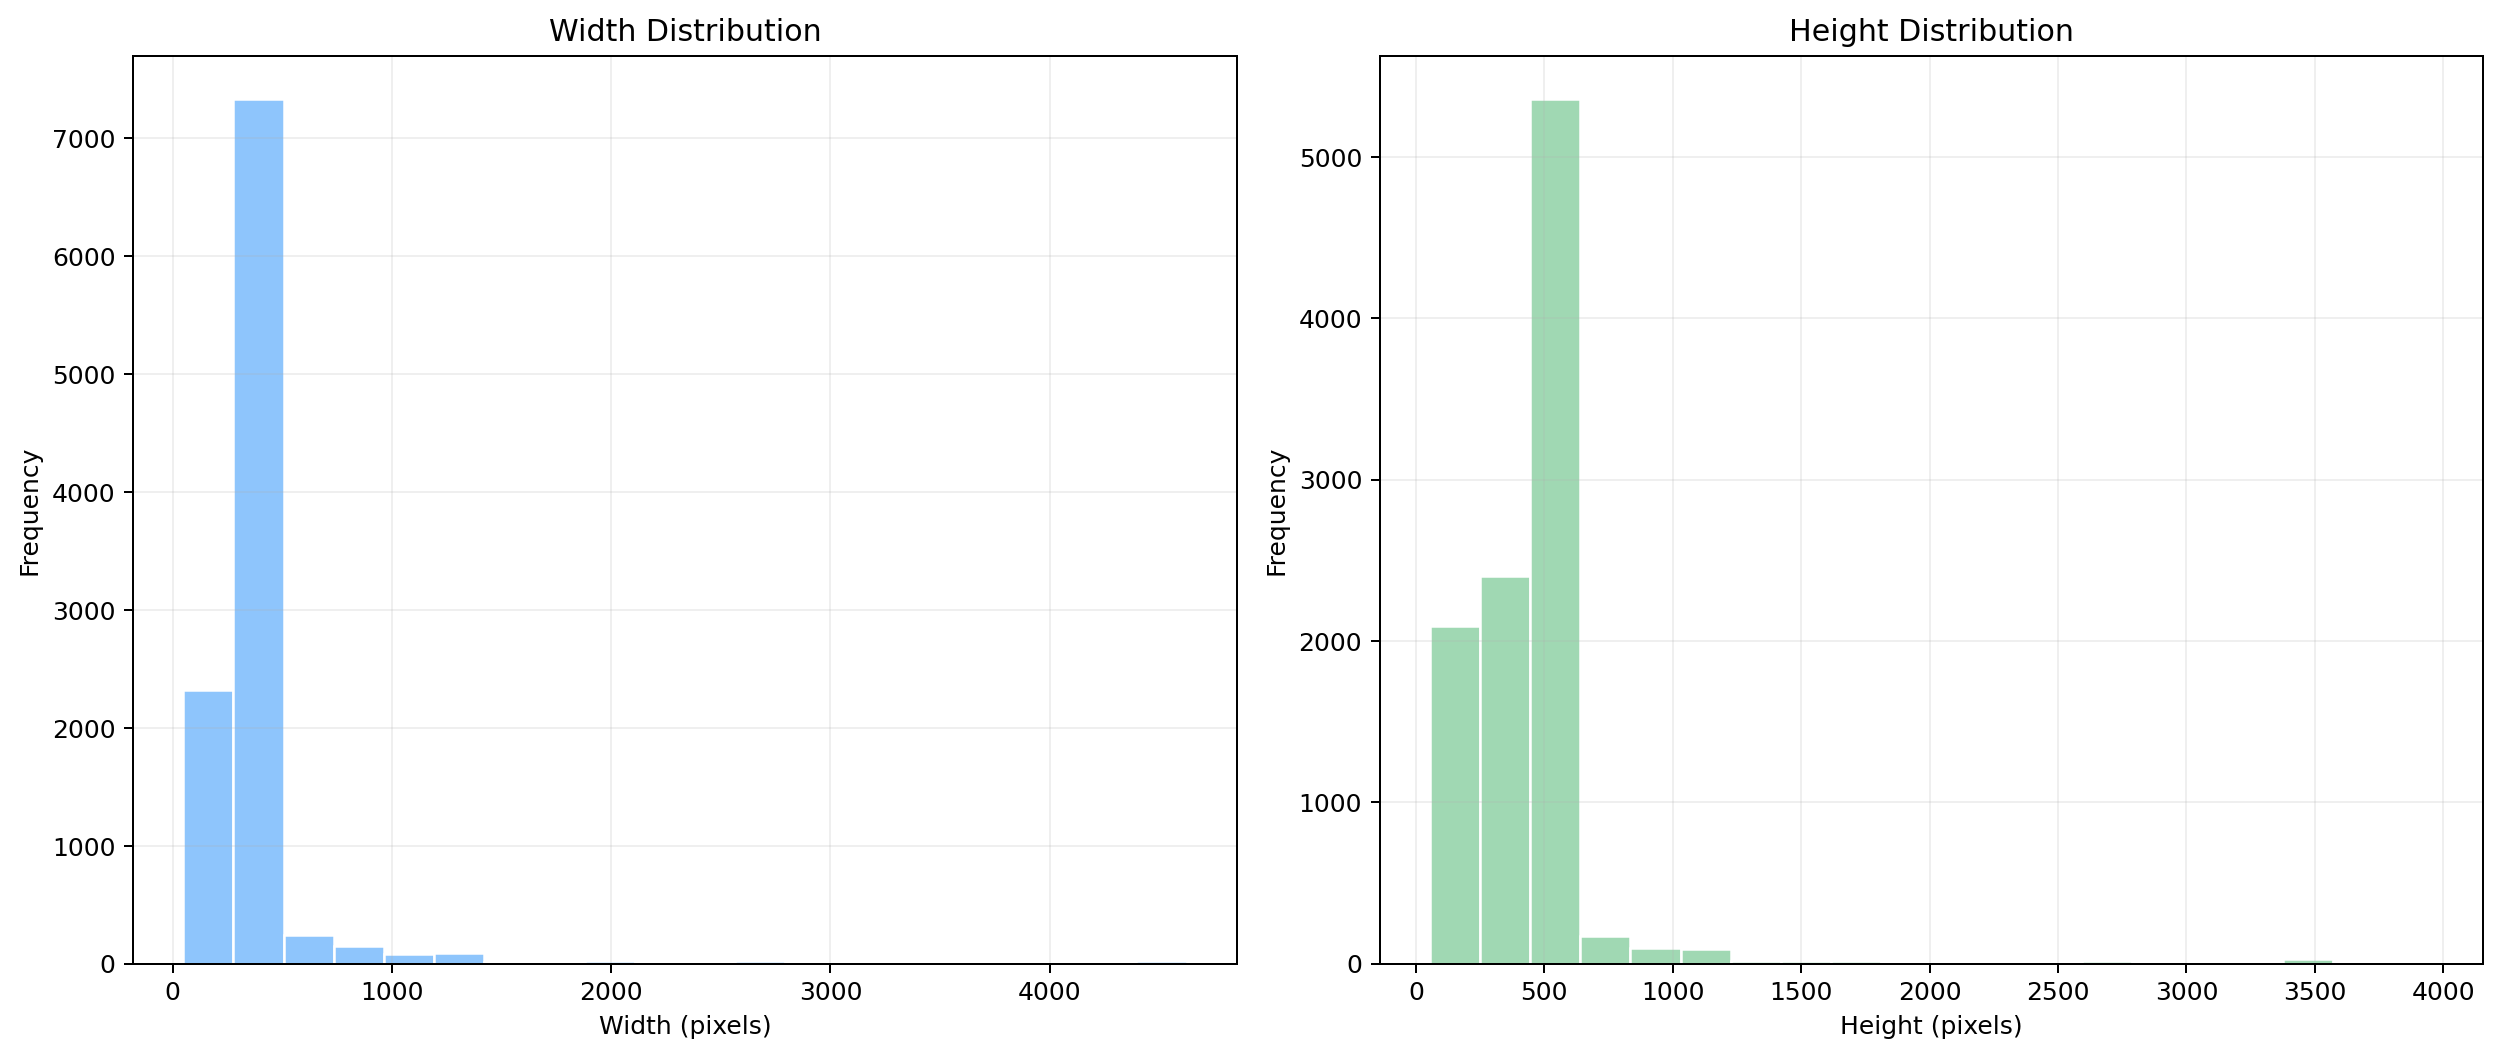
\includegraphics[width=0.82\textwidth]{image_size_distribution.png}
    \caption{Distribution of image sizes in the cleaned training set. The variability in raw resolution motivates a standardized preprocessing pipeline before training.}
\end{figure}

\begin{figure}[htbp]
    \centering
    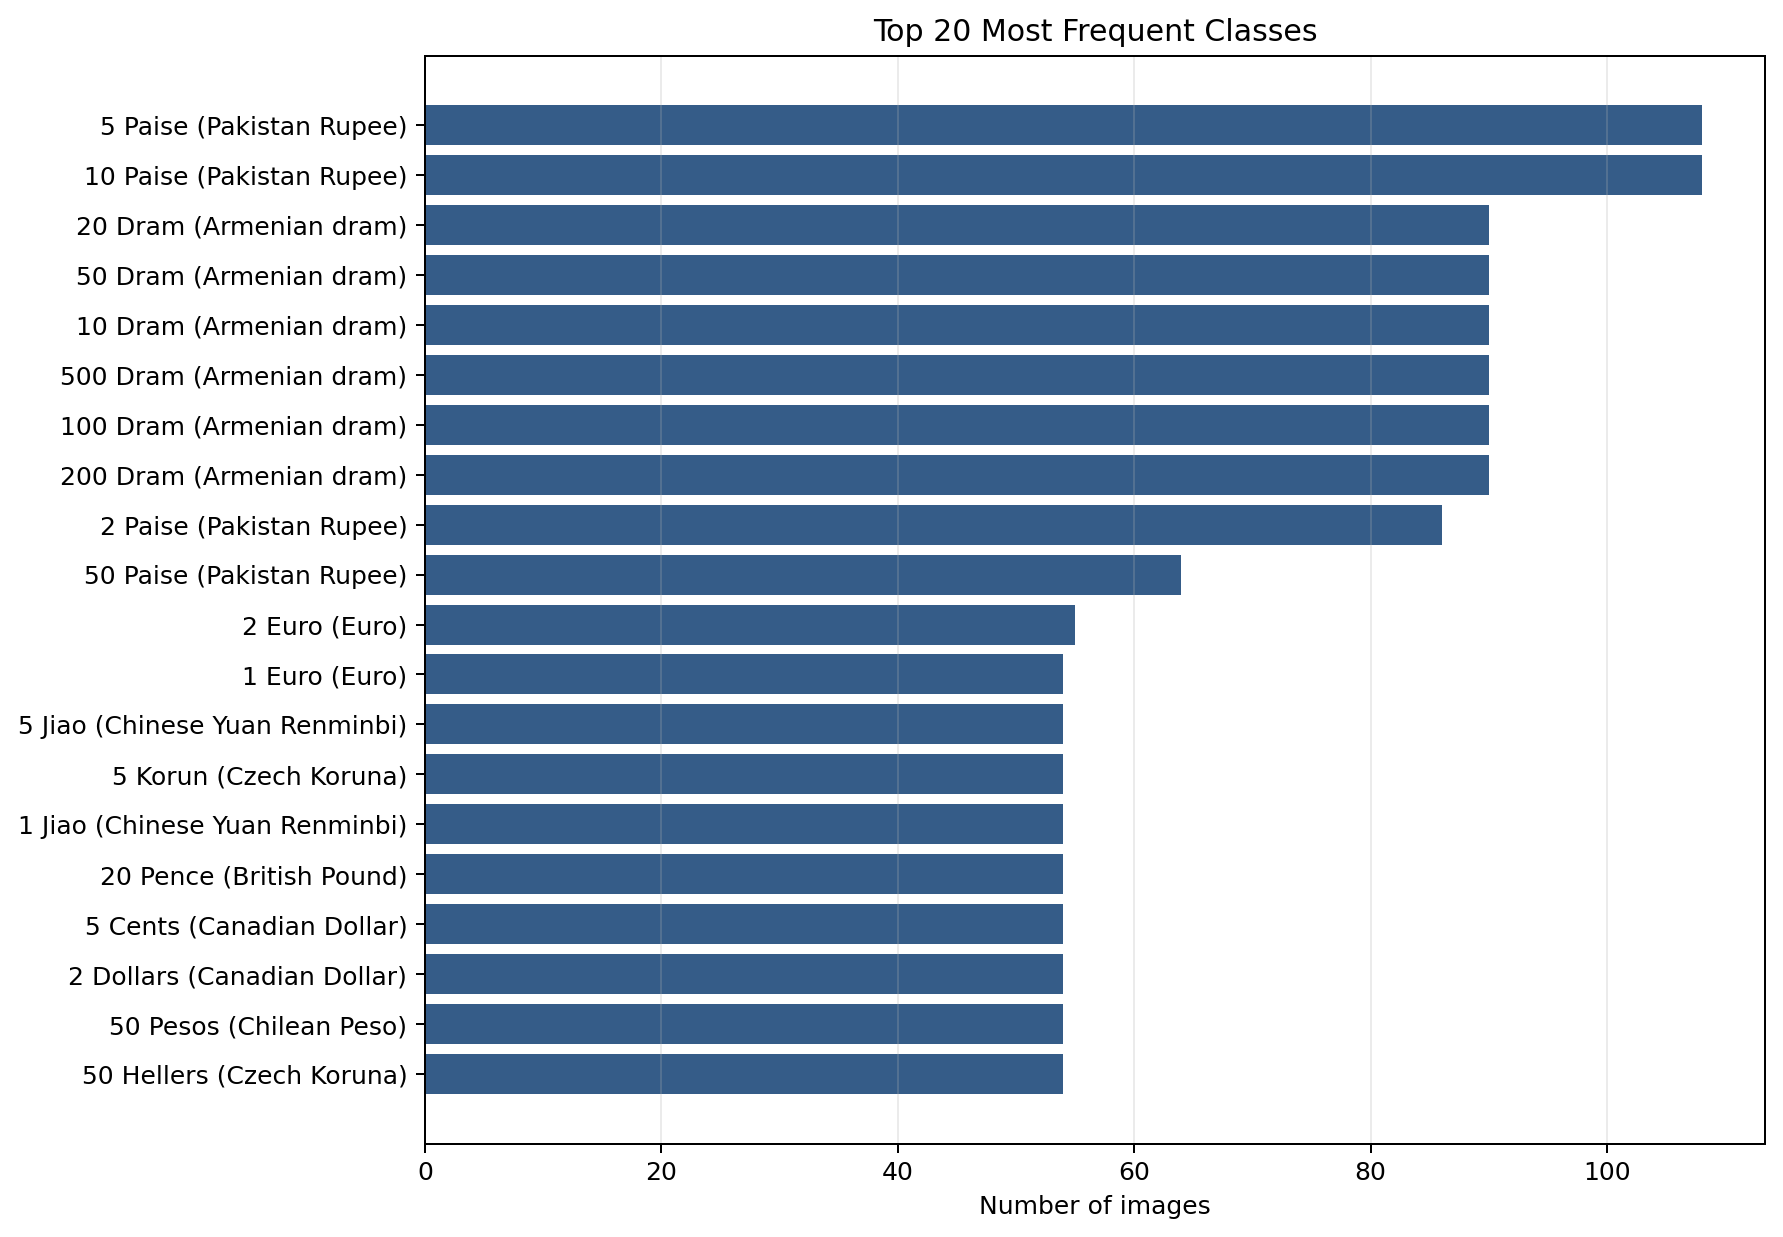
\includegraphics[width=0.9\textwidth]{class_distribution_top20.png}
    \caption{Top-20 most frequent classes in the training data. The imbalance visible here supports the use of weighted sampling and macro-aware evaluation metrics.}
\end{figure}

\section{Baseline Version And Its Limits}
Pretrained AlexNet, an 80/20 stratified split, data augmentation, weighted sampling, and a two-stage optimization strategy. However, its reported training schedule remained relatively short, with only 2 warm-up epochs on the classifier head followed by 3 fine-tuning epochs on the full network.

That earlier version produced solid results, reaching a validation accuracy of 0.7043, a top-5 accuracy of 0.8741, a macro-F1 of 0.6650, and a balanced accuracy of 0.6803. It also produced a Kaggle submission with public score 0.71918 and private score 0.71606.

Even so, there were still clear improvement opportunities:
\begin{itemize}[leftmargin=1.4em]
    \item the total training budget was still modest for a 315-class problem,
    \item the fine-tuning phase could be made more gradual and better controlled,
    \item stopping criteria could be improved to avoid wasting epochs once validation stopped improving,
\end{itemize}

\section{Improvements}
The current codebase introduces a set of concrete improvements that make the system easier to justify scientifically.

\subsection{Longer Two-Stage Training Schedule}
The most important modification concerns the number of epochs. The current configuration defines:
\begin{itemize}[leftmargin=1.4em]
    \item \textbf{4 warm-up epochs} for the classifier head with frozen convolutional features,
    \item \textbf{10 fine-tuning epochs} for the full model after unfreezing the feature extractor.
\end{itemize}

This means that the updated pipeline can train for up to 14 epochs in total. The purpose of this change is straightforward: the classifier head is given more time to adapt to the 315 target classes before the pretrained feature extractor is fully adjusted, and the fine-tuning stage is long enough to capture class-specific details of coins such as texture, relief, border shape, and inscriptions.

\subsection{Early Stopping To Control Overfitting}
Increasing the maximum number of epochs is useful only if overfitting is controlled. The patience mechanism stops training when validation accuracy no longer improves for several consecutive epochs, which protects the run from unnecessary computation and reduces the risk of keeping a degraded model.

In addition, the code keeps track of the best validation checkpoint and reloads it before the final evaluation. This is a better protocol than blindly using the very last epoch.

\subsection{Improved Optimization Strategy}
The optimizer is AdamW, which is generally more stable than basic SGD for this kind of transfer-learning setup. I also use a cosine annealing scheduler inside each training stage. This makes the learning rate decay progressively instead of remaining fixed during the entire stage.

The logic is the following:
\begin{itemize}[leftmargin=1.4em]
    \item during head warm-up, only the classifier is optimized,
    \item during full fine-tuning, the convolutional features use a smaller learning rate than the classifier,
    \item the scheduler gradually reduces the learning rate inside each stage.
\end{itemize}

This differential learning-rate design is technically sound because the pretrained convolutional backbone should change more cautiously than the randomly reinitialized final classification layer.

\subsection{Data Augmentation}
\begin{itemize}[leftmargin=1.4em]
    \item random resized crop to 224 with scale range $(0.7, 1.0)$ and ratio range $(0.9, 1.1)$,
    \item random rotation up to 20 degrees,
    \item moderate color jitter on brightness, contrast, saturation, and hue,
    \item ImageNet normalization matching pretrained AlexNet.
\end{itemize}

An important detail is that random erasing is currently disabled in the code. This is a meaningful adjustment rather than a regression: on natural-image tasks, random erasing often helps, but for coin recognition it can hide precisely the fine border details, symbols, and text that distinguish visually similar classes. Disabling it therefore reflects a more task-aware choice.

\subsection{Handling Class Imbalance}
This is an improvement because the dataset is unbalanced, with classes ranging from 13 to 108 examples. Weighted sampling gives rare classes more opportunities to be seen during training and is therefore aligned with the use of macro-F1 and balanced accuracy for evaluation.

\subsection{Regularization And Stability}
Label smoothing is at 0.1. This is a reasonable setting for a fine-grained visual classification problem in which many classes are similar. The training loop also applies gradient clipping, which adds another layer of optimization stability.

\subsection{Reproducibility}

\begin{itemize}[leftmargin=1.4em]
    \item \code{classification\_report.json} for class-wise metrics,
    \item \code{validation\_metrics.json} for the final aggregate results,
    \item \code{training\_history.png} for the learning curves,
    \item \code{submission.csv} for Kaggle evaluation.
\end{itemize}

I also used a fixed random seed and print the full run configuration at launch, which makes the experimental setup easier to reproduce and compare across versions.


\section{Experimental Protocol}
The current experimental protocol can be summarized as follows:
\begin{enumerate}[leftmargin=1.6em]
    \item load the CSV annotations and build the image index,
    \item filter invalid images before any split,
    \item encode the 315 class labels,
    \item create a stratified 80/20 train/validation split,
    \item initialize AlexNet with pretrained ImageNet weights,
    \item replace the final classification layer to match the number of classes,
    \item train the classifier head for up to 4 epochs with learning rate $5 \times 10^{-4}$,
    \item unfreeze the network and fine-tune for up to 10 more epochs with learning rate $10^{-4}$,
    \item use weighted sampling, label smoothing, gradient clipping, and cosine annealing,
    \item stop early if validation accuracy does not improve for 4 epochs,
    \item reload the best checkpoint, evaluate on validation, and export a Kaggle submission.
\end{enumerate}

\section{Results}
The first try already documented a validation accuracy of 70.43\%, top-5 accuracy of 87.41\%, macro-F1 of 0.6650, and balanced accuracy of 68.03\%. It also documented a Kaggle result of 0.71918 public and 0.71606 private.

The latest submission improved the Kaggle result significantly, reaching a public score of 0.82839 and a private score of 0.77067.

Extending the training budget makes sense because transfer learning on a 315-class dataset may still need several epochs before the model fully adapts. Early stopping prevents this larger budget from turning into uncontrolled overfitting. Likewise, preserving weighted sampling and label smoothing is good for a fine-grained imbalanced classification problem.

The gap between public and private scores also shows that the model still faces some generalization difficulty, which is expected in a task with many visually similar classes. Even so, the private score improvement compared with the earlier submission indicates that the updated training strategy was beneficial overall.

\begin{figure}[!ht]
    \centering
    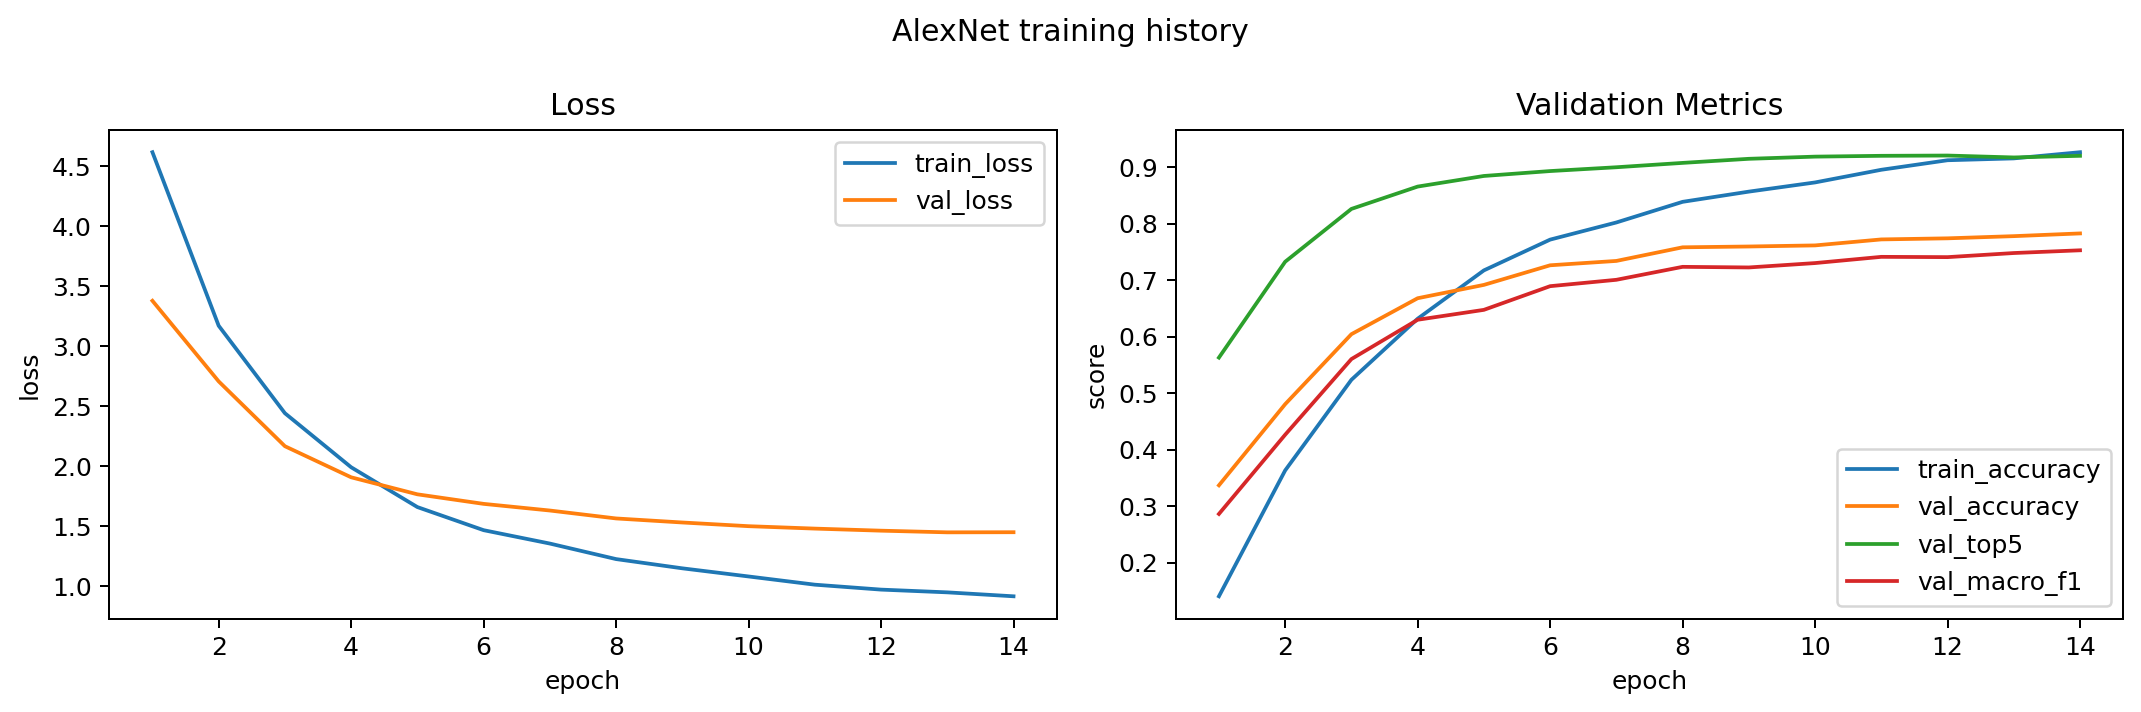
\includegraphics[width=0.82\textwidth]{training_history.png}
    \caption{Training and validation curves across the two-stage AlexNet optimization schedule. The learning dynamics support the benefit of the longer budget combined with early stopping.}
\end{figure}

\section{Critical Discussion}
Several limitations remain.

First, the task is intrinsically difficult because many coin classes differ only by subtle symbols, inscriptions, year markings, or metallic texture. AlexNet can solve a large part of the problem, but its feature extractor is less modern than contemporary architectures.

Second, all images are resized to the AlexNet input size of 224 x 224. This is standard and practical, but it may also suppress some very fine discriminative details present in high-resolution coin photographs.



\section{Conclusion}
The main changes are the move from a short 5-epoch schedule to a longer two-stage training budget of up to 14 epochs, the addition of early stopping, the use of cosine annealing inside each training stage, better checkpoint handling, more careful experiment tracking, and a refined view of augmentation in which random erasing is disabled because it may hide useful coin details.

The latest Kaggle submission also supports the relevance of these changes, with a clear improvement from the earlier result to a public score of 0.82839 and a private score of 0.77067. This strengthens the argument that the system was not only modified, but genuinely improved.


\end{document}
